\chapter{\label{app:isc-results}Appendix \textemdash\ Indian subcontinent model results}

\minitoc

\section{\label{app:isc-results-cp-dist-cont}Continuous predictor distributions by study}

The following figures show the distributions of continuous candidate predictors by ISC study. For each predictor, two plots are provided: (i) [left plot] histograms normalised within each study (each study's bars sum to the same area), and (ii) [right plot] histograms normalised across all studies to reflect their relative sample sizes. The y-axis labels also indicate the amount of missing data. Height, weight, and haemoglobin are included because they are used to derive the categorical predictors for malnutrition and anaemia, even though they are not predictors themselves.

Fever duration and the laboratory tests are log-transformed given their marked right-skewed distributions.

\begin{tabular}{ll}
  \toprule
  \textbf{Variable}                & \textbf{Figure reference}  \\
  \midrule
  Age                              & \ref{fig:isc_age_comb}     \\
  Height                           & \ref{fig:isc_height_comb}  \\
  Weight                           & \ref{fig:isc_weight_comb}  \\
  BMI                              & \ref{fig:isc_height_comb}  \\
  BMI-for-age z-score              & \ref{fig:isc_bmiz_comb}    \\
  Weight-for-height z-score        & \ref{fig:isc_wfh_comb}     \\
  Spleen size                      & \ref{fig:isc_ss_comb}      \\
  Fever duration (log scale)       & \ref{fig:isc_fd_log_comb}  \\
  White blood cell (log scale)     & \ref{fig:isc_wbc_log_comb} \\
  Platelets (log scale)            & \ref{fig:isc_plt_log_comb} \\
  Haemoglobin (log scale)          & \ref{fig:isc_hb_log_comb}  \\
  Alanine transaminase (log scale) & \ref{fig:isc_alt_log_comb} \\
  Creatinine (log scale)           & \ref{fig:isc_cr_log_comb}  \\
  \bottomrule
\end{tabular}

\newgeometry{left=1cm, bottom=2.5cm, right=2cm, top=3cm}

% AGE
% cp /Users/jameswilson/proj/vl_model_isc/figures/dist/age_comb.pdf figures/ch5/isc_age_comb.pdf
\begin{landscape}
  \begin{figure}[tb]
    \centering
    \includegraphics[width=1.35\textwidth]{figures/ch5/isc_age_comb.pdf}
    \caption{Distribution of age across studies from the Indian subcontinent. Missing age data described by study.}
    \label{fig:isc_age_comb}
  \end{figure}
\end{landscape}

% HEIGHT
% cp /Users/jameswilson/proj/vl_model_isc/figures/dist/height_comb.pdf figures/ch5/isc_height_comb.pdf
\begin{landscape}
  \begin{figure}[tb]
    \centering
    \includegraphics[width=1.35\textwidth]{figures/ch5/isc_height_comb.pdf}
    \caption{Distribution of height across studies from the Indian subcontinent. Missing data described by study.}
    \label{fig:isc_height_comb}
  \end{figure}
\end{landscape}

% WEIGHT
% cp /Users/jameswilson/proj/vl_model_isc/figures/dist/weight_comb.pdf figures/ch5/isc_weight_comb.pdf
\begin{landscape}
  \begin{figure}[tb]
    \centering
    \includegraphics[width=1.35\textwidth]{figures/ch5/isc_weight_comb.pdf}
    \caption{Distribution of weight across studies from the Indian subcontinent. Missing data described by study.}
    \label{fig:isc_weight_comb}
  \end{figure}
\end{landscape}

% BMI
% cp /Users/jameswilson/proj/vl_model_isc/figures/dist/bmi_comb.pdf figures/ch5/isc_bmi_comb.pdf
\begin{landscape}
  \begin{figure}[tb]
    \centering
    \includegraphics[width=1.35\textwidth]{figures/ch5/isc_bmi_comb.pdf}
    \caption{Distribution of BMI across studies from the Indian subcontinent. Including only participants aged 19 and over (Pandey 2017 excluded). Missing data described by study.}
    \label{fig:isc_bmi_comb}
  \end{figure}
\end{landscape}

% BMI-FOR-AGE Z SCORE
% cp /Users/jameswilson/proj/vl_model_isc/figures/dist/bmiz_comb.pdf figures/ch5/isc_bmiz_comb.pdf
\begin{landscape}
  \begin{figure}[tb]
    \centering
    \includegraphics[width=1.35\textwidth]{figures/ch5/isc_bmiz_comb.pdf}
    \caption{Distribution of BMI-for-age z score across studies from the Indian subcontinent. Including only participants aged from 5--18, inclusive. Missing data described by study.}
    \label{fig:isc_bmiz_comb}
  \end{figure}
\end{landscape}

% WEIGHT-FOR-HEIGHT Z SCORE
% cp /Users/jameswilson/proj/vl_model_isc/figures/dist/wfh_comb.pdf figures/ch5/isc_wfh_comb.pdf
\begin{landscape}
  \begin{figure}[tb]
    \centering
    \includegraphics[width=1.35\textwidth]{figures/ch5/isc_wfh_comb.pdf}
    \caption{Distribution of weight-for-height z score across studies from the Indian subcontinent. Including only participants aged under 5. Missing data described by study.}
    \label{fig:isc_wfh_comb}
  \end{figure}
\end{landscape}

% SPLEEN SIZE
% cp /Users/jameswilson/proj/vl_model_isc/figures/dist/ss_comb.pdf figures/ch5/isc_ss_comb.pdf
\begin{landscape}
  \begin{figure}[tb]
    \centering
    \includegraphics[width=1.35\textwidth]{figures/ch5/isc_ss_comb.pdf}
    \caption{Distribution of spleen size across studies from the Indian subcontinent. Missing data described by study.}
    \label{fig:isc_ss_comb}
  \end{figure}
\end{landscape}

% % FEVER DURATION
% % cp /Users/jameswilson/proj/vl_model_isc/figures/dist/fd_comb.pdf figures/ch5/isc_fd_comb.pdf
% \begin{landscape}
%     \begin{figure}[tb]
%         \centering
%         \includegraphics[width=1.50\textwidth]{figures/ch5/isc_fd_comb.pdf}
%         \caption{Distribution of fever duration across studies from the Indian subcontinent. Missing data described by study.}
%         \label{fig:isc_fd_comb}
%     \end{figure}
% \end{landscape}

% FEVER DURATION LOG SCALE
% cp /Users/jameswilson/proj/vl_model_isc/figures/dist/fd_log_comb.pdf figures/ch5/isc_fd_log_comb.pdf
\begin{landscape}
  \begin{figure}[tb]
    \centering
    \includegraphics[width=1.35\textwidth]{figures/ch5/isc_fd_log_comb.pdf}
    \caption{Distribution of fever duration (log scale) across studies from the Indian subcontinent. Missing data described by study.}
    \label{fig:isc_fd_log_comb}
  \end{figure}
\end{landscape}


% WBC LOG SCALE
% cp /Users/jameswilson/proj/vl_model_isc/figures/dist/wbc_log_comb.pdf figures/ch5/isc_wbc_log_comb.pdf
\begin{landscape}
  \begin{figure}[tb]
    \centering
    \includegraphics[width=1.35\textwidth]{figures/ch5/isc_wbc_log_comb.pdf}
    \caption{Distribution of white blood cell count (log scale) across studies from the Indian subcontinent. Missing data described by study.}
    \label{fig:isc_wbc_log_comb}
  \end{figure}
\end{landscape}

% PLATELETS LOG SCALE
% cp /Users/jameswilson/proj/vl_model_isc/figures/dist/plt_log_comb.pdf figures/ch5/isc_plt_log_comb.pdf

\begin{landscape}
  \begin{figure}[tb]
    \centering
    \includegraphics[width=1.35\textwidth]{figures/ch5/isc_plt_log_comb.pdf}
    \caption{Distribution of platelet count (log scale) across studies from the Indian subcontinent. Missing data described by study.}
    \label{fig:isc_plt_log_comb}
  \end{figure}
\end{landscape}

% HAEMOGLOBIN LOG SCALE
% cp /Users/jameswilson/proj/vl_model_isc/figures/dist/hb_log_comb.pdf figures/ch5/isc_hb_log_comb.pdf

\begin{landscape}
  \begin{figure}[tb]
    \centering
    \includegraphics[width=1.35\textwidth]{figures/ch5/isc_hb_log_comb.pdf}
    \caption{Distribution of haemoglobin (log scale) across studies from the Indian subcontinent. Missing data described by study.}
    \label{fig:isc_hb_log_comb}
  \end{figure}
\end{landscape}

% ALT LOG SCALE
% cp /Users/jameswilson/proj/vl_model_isc/figures/dist/alt_log_comb.pdf figures/ch5/isc_alt_log_comb.pdf

\begin{landscape}
  \begin{figure}[tb]
    \centering
    \includegraphics[width=1.35\textwidth]{figures/ch5/isc_alt_log_comb.pdf}
    \caption{Distribution of alanine transaminase (ALT, log scale) across studies from the Indian subcontinent. Missing data described by study.}
    \label{fig:isc_alt_log_comb}
  \end{figure}
\end{landscape}

% CREATININE LOG SCALE
% cp /Users/jameswilson/proj/vl_model_isc/figures/dist/cr_log_comb.pdf figures/ch5/isc_cr_log_comb.pdf

\begin{landscape}
  \begin{figure}[tb]
    \centering
    \includegraphics[width=1.35\textwidth]{figures/ch5/isc_cr_log_comb.pdf}
    \caption{Distribution of creatinine (log scale) across studies from the Indian subcontinent. Missing data described by study.}
    \label{fig:isc_cr_log_comb}
  \end{figure}
\end{landscape}

\restoregeometry

\section{\label{app:results-cp-dist-cat}Categorical predictor distributions by study}

\newgeometry{left=1cm, bottom=2.5cm, right=1.5cm, top=3cm}

% cp /Users/jameswilson/proj/vl_model_isc/figures/dist/comb_discrete.pdf figures/ch5/isc_comb_discrete.pdf
\begin{landscape}
  \begin{figure}[tb]
    \centering
    \includegraphics[width=1.35\textwidth]{figures/ch5/isc_comb_discrete.pdf}
    \caption{Distribution of categorical predictors by study. Missing data excluded from stacked bar charts for malnutrition, parasite grade. Where aspirates were performed, the source was never missing. NA: unable to show distribution as all study-specific data are missing. MF: miltefosine; SDA: single-dose liposomal amphotericin B}
    \label{fig:isc_comb_dist_cat}
  \end{figure}
\end{landscape}

\restoregeometry

\section{\label{app:isc-results-cp-ass-cont-cont}Pooled continuous-continuous predictor associations}

\newgeometry{left=1cm, bottom=2.5cm, right=1.5cm, top=3cm}
%cp /Users/jameswilson/proj/vl_model_isc/figures/dist/ass/cont_cont.pdf figures/ch5/isc_cont_cont.pdf

\begin{landscape}
  \begin{figure}[tb]
    \centering
    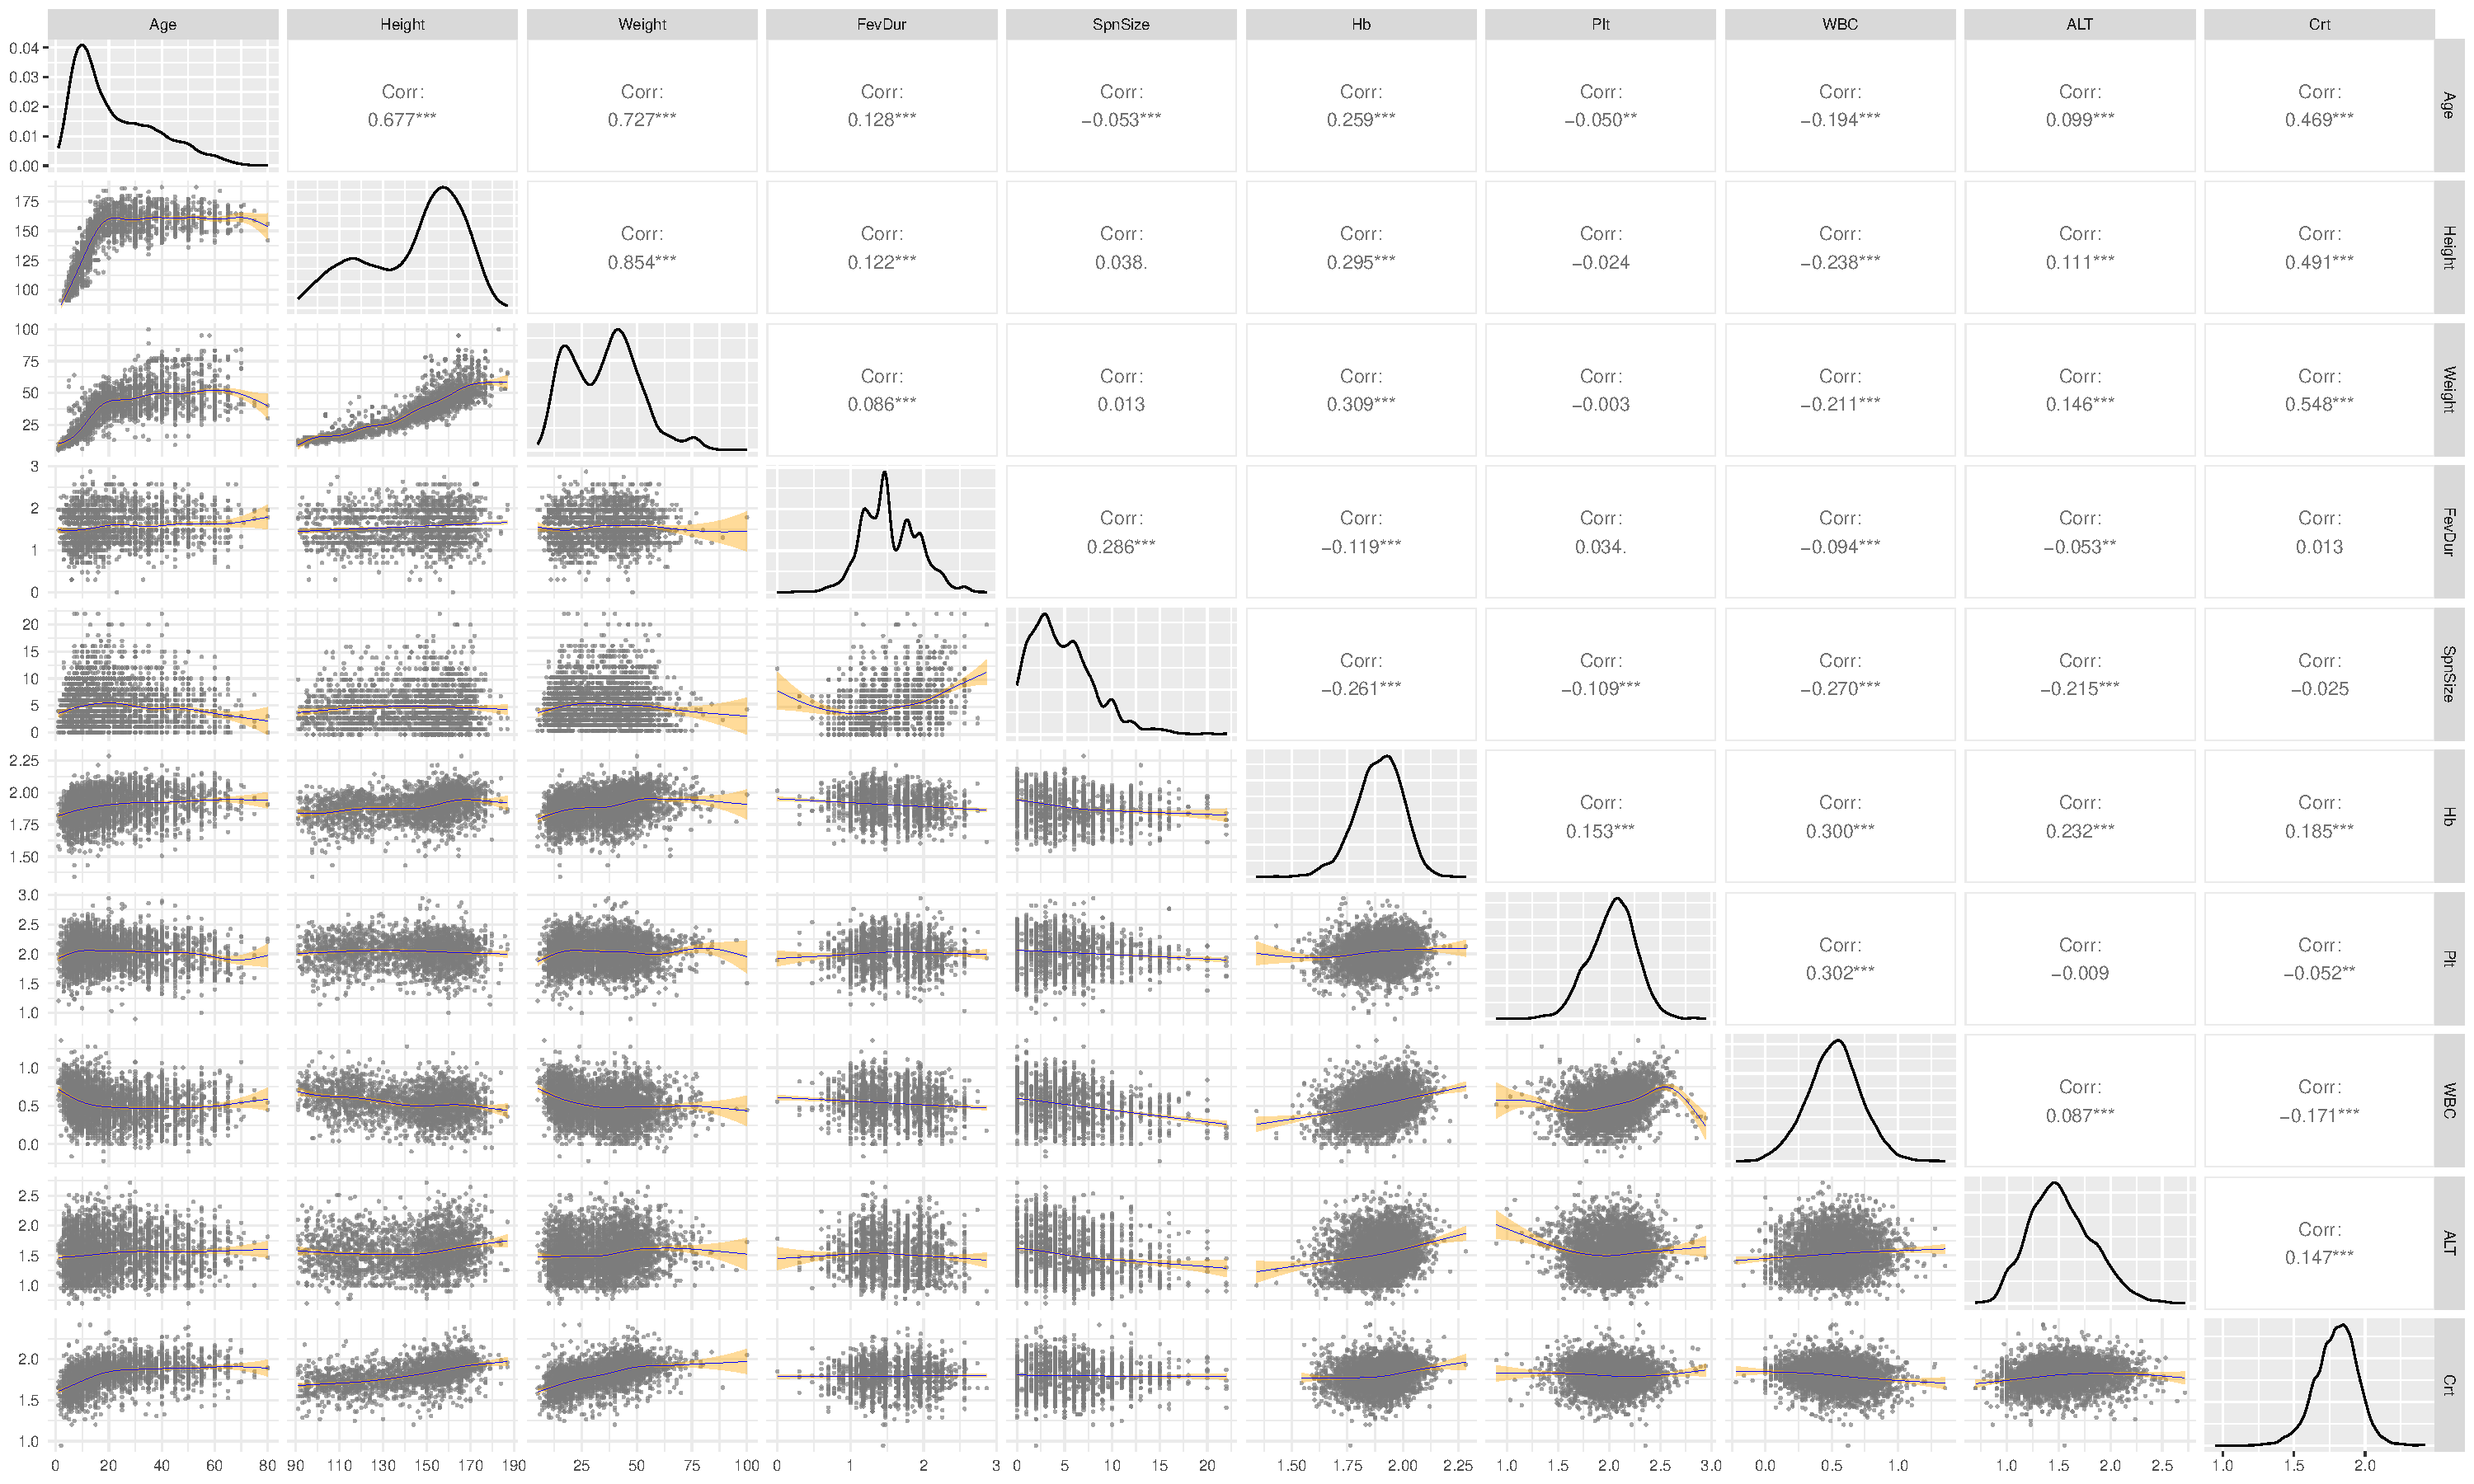
\includegraphics[width=1.34\textwidth]{figures/ch5/isc_cont_cont.pdf}
    \caption{Correlation between continuous variables. For scatter plots, a univariable generalised additive model is fitted (blue line) with 95\% confidence interval ribbon filled (orange area). Pearson correlation coefficients are presented, `***' p<0.001; `**' p<0.01; `*' p<0.05, `.' p<0.10. Age: years; Height: cm; Weight: kg; FevDur: duration of fever, log10(days); SpnSize: spleen size (cm); Hb: haemoglobin, log10(g/L); Plt: platelets, log10($\times10^9/L$); WBC: white blood cells log10($\times10^9/L$); ALT: alanine aminotransferase, log10(U/L); Cr: creatinine log10($\mu$mol/L).}
    \label{fig:isc_cont_cont}
  \end{figure}
\end{landscape}

\restoregeometry

\section{\label{app:isc-results-cp-ass-cont-cat}Pooled continuous-categorical predictor associations}

\newgeometry{left=1cm, bottom=2.5cm, right=1.5cm, top=3cm}
%cp /Users/jameswilson/proj/vl_model_isc/figures/dist/ass/cont_cat.pdf figures/ch5/isc_cont_cat.pdf

\begin{landscape}
  \begin{figure}[tb]
    \centering
    \includegraphics[width=1.34\textwidth]{figures/ch5/isc_cont_cat.pdf}
    \caption{Correlation between continuous and categorical variables. FevDur and laboratory tests axes transformed to log10 scale. Age: years; Height: cm; Weight: kg; FevDur: duration of fever, days; SpnSize: spleen size, cm; Hb: haemoglobin, g/L; Plt: platelets, $\times10^9/L$; WBC: white blood cells $\times10^9/L$; ALT: alanine aminotransferase, U/L; Cr: creatinine $\mu$mol/L.}
    \label{fig:isc_cont_cat}
  \end{figure}
\end{landscape}

\restoregeometry
